\documentclass{article}
\usepackage{/opt/asta/share/90sek/kurzinfo_red}
\newfont{\klitzeklein}{cmss10 at 8.5pt}

\newcommand{\frage}[1]{\vspace*{1ex}

\textbf{#1}\\
}

\verantwortlich{J. Sch"ope}
\druck{AStA Druckerei}
\auflage{ca. 5000}
\ausgabennummer{168} %% BITTE NACHSEHEN
\begin{document}
%<doppelseite>
%% DATUM KORRIGIEREN !!!%%%%

\begin{vorderseite}{Stand September 2012}{BAf"oG-Kurzinfo} %erste Seite, Datum und Ueberschrift (90 Sekunden extra gibts ja auch\ldots)
\zweispalten{.5\linewidth}
{%Kommentar: linke Spalte 
\vspace{-4pt}
\begin{artikel}{}
\vspace{-16pt}
Neben der Entscheidung, welches Fach Du an welcher Hochschule studieren m"ochtest, stellt sich zum Studienanfang nat"urlich auch die Frage der Studienfinanzierung. Dabei geht es im Wesentlichen um das Aufbringen der allgemeinen Lebenshaltungskosten, die sp"atestens jetzt, wo Du hoffentlich eine eigene Wohnung in Aachen gefunden hast, auch auf Dich zukommen.

F"ur Studierende, die w"ahrend des Studiums finanziell nicht von ihren Eltern unterst"utzt werden k"onnen, gibt es die Bundesausbildungsf"orderung -- kurz auch BAf"oG genannt (von BundesAusbildungsf"orderungsGesetz).\\

Dieses Info-Blatt soll einen "Uberblick und Antworten auf die wichtigsten Fragen geben, die sich viele ErstsemesterInnen stellen. Da das BAf"oG Gesetz sehr komplex ist und es viele Ausnahmeregelungen gibt, k"onnen wir hier nur die Standard-F"alle beschreiben. F"ur detailliertere Fragen oder f"ur Probleme bei der Beantragung steht Dir im AStA eine BAf"oG-Beratung zur Verf"ugung.

Au"serdem findest Du auf der R"uckseite eine Aufstellung der wichtigsten Anlaufstellen, die zu der Antragstellung, dem BAf"oG-Bescheid oder der R"uckzahlung informieren oder beraten k"onnen.
\end{artikel}

\begin{artikel}{Antragstellung}

\frage{Was geh"ort in den Erstantrag?}
F"ur die Antragstellung musst Du einige Antragsformulare ausf"ullen. Diese Antr"age findest Du im Internet unter: \url{http://www.studentenwerk-aachen.de/bafoeg/bafoeg/download/start.asp} oder beim BAf"oG Amt in der Peterstra"se 44 - 46 in Aachen.

Alle BAf"oG-Empf"angerInnen m"ussen das Formblatt 1 und das Zusatzblatt zum Formblatt 1 ausf"ullen. Solltest Du elternabh"angiges BAf"oG bekommen (was der Regelfall ist), musst Du f"ur Deine Eltern das Formblatt 3 plus den Lohnsteuerbescheid von vor zwei Jahren abgeben. Sollten Deine Eltern nicht gemeinsam zur Lohnsteuer veranlagt werden, muss das Formblatt pro Elternteil mit Einkommen einmal ausgef"ullt werden. Wenn Du eine eigene Wohnung hast, musst Du noch eine Mietbescheinigung einreichen. Au"ser den Formbl"attern geh"ort noch ein Krankenversicherungsnachweis und eine Studienbescheinigung in den Antrag.

Falls Du keine deutsche Staatsangeh"origkeit hast, musst Du zus"atzlich noch das Formblatt 4 abgeben.

\frage{Wann sollte ich meinen Erstantrag abgeben?}
Am besten ca. drei Monate vor Beginn des ersten Semesters. Damit stellst Du sicher, dass "uber Deinen Antrag rechtzeitig entschieden wird, um zum Anfang des ersten Semesters F"orderung zu erhalten.

Sp"atestens musst Du den Antrag bis zum Ende des ersten Studienmonats stellen. Allerdings ist davon stark abzuraten, schlie"slich kann die Bearbeitung Deines Antrags eine ganze Weile dauern.

Du kannst auch noch nach Ende des ersten Studienmonats einen Antrag stellen, hast aber dann keinen Anspruch mehr auf eine Nachzahlung f"ur die vergangenen Monate.

\frage{Wie lange dauert die Entscheidung "uber meinen Antrag im Normalfall?}
Hast Du Deinen Antrag fr"uhzeitig abgegeben (ca. 3 Monate vor Beginn des ersten Semesters), sollte sp"atestens zum Semester-
\end{artikel}

}
{%Kommentar: rechte Spalte
\begin{artikel}{}
\vspace{-20pt}
beginn ein Bescheid in Deinem Briefkasten sein. Vorausgesetzt nat"urlich, Du hast auch alle Nachweise fr"uhzeitig eingereicht.

Falls Du zwei Wochen danach noch keinen Bescheid hast, solltest Du Dich beim BAf"oG-Amt melden. Gibst Du Deinen Antrag erst wenige Wochen vor Semesterbeginn ab, musst Du damit rechnen eventuell mehrere Monate warten zu m"ussen. Du erh"altst dann eine Nachzahlung. Das BAf"oG-Amt gibt sich zwar bei Erstantr"agen alle M"uhe, schnell zu bescheiden. Wenn aber viele Antr"age sehr kurzfristig gestellt werden, dauert es nat"urlich recht lange.

\frage{Ich werde den Erstantrag samt Nachweisen nicht rechtzeitig abgeben k"onnen. Was muss ich beachten?}
Falls Du es nicht mehr bis Ende des ersten Studienmonats schaffst: Stell in jedem Fall einen formlosen Antrag beim BAf"oG-Amt, um Deinen Anspruch ab Studienbeginn nicht zu verlieren. Es reicht ein Brief mit dem Inhalt:

"`Hiermit beantrage ich, \{Vorname Nachname\}, Leistungen nach dem BAf"oG."'

Kannst Du auch die Frist zur Abgabe der restlichen Unterlagen nicht einhalten, die Dir vom BAf"oG-Amt auf Deinen "`Kurzantrag"' hin gesetzt wurde, sprich dies vorher mit dem Amt ab.
\end{artikel}

\begin{artikel}{Der Bescheid}

Wenn das BAf"oG-Amt Deinen Antrag bearbeitet hat, bekommst Du den sogenannten BAf"oG Bescheid zugesendet. In diesem Bescheid ist aufgef"uhrt, wie viel Geld Du im kommenden Jahr monatlich an BAf"oG bekommst. Au"serdem kannst Du sehen, wie viel Geld Du laut BAf"oG Gesetz pro Monat brauchst und wie viel Dir Deine Eltern geben m"ussen.

\frage{Was mache ich, wenn ich glaube, dass sich das BAf"oG Amt bei der Berechnung vertan hat?}
Solltest Du das Gef"uhl haben, dass etwas mit Deinem Bescheid nicht stimmt, such m"oglichst schnell eine Beratungsstelle auf und vergewissere Dich, ob die Berechnung richtig ist. Du solltest Dich damit beeilen, da Du nur einen Monat Zeit hast gegen den BAf"oG Bescheid Widerspruch einzulegen.

\frage{Was mache ich, wenn meine Eltern nicht bereit sind ihren Anteil zu zahlen?}
In einem solchen Fall musst Du dem Amt f"ur Ausbildungsf"orderung glaubhaft machen, dass Deine Eltern nicht bereit sind, den Anteil zu "ubernehmen, den sie zu Deinem Bedarf beisteuern m"ussen. Dann ist es m"oglich, eine BAf"oG-Vorausleistung zu erhalten. Du bekommst dann das gesamte ben"otigte Geld. Dabei gehen Deine Unterhaltsanspr"uche auf das BAf"oG-Amt "uber, das sich wiederum bem"uhen wird, das Geld von Deinen Eltern einzutreiben. Dieses Verfahren ist meistens mit der Anh"orung Deiner Eltern verbunden und hat f"ur sie rechtliche Konsequenzen. Du solltest nat"urlich alles versuchen, um dieses Problem mit Deinen Eltern anderweitig zu kl"aren. In schwierigeren F"allen hilft es vielleicht, Sie auf obige Regelung hinzuweisen.
\end{artikel}


}
%\fcolorbox{black}{light}{\parbox{\linewidth}{\textbf{\footnotesize Haftungsausschluss}%
%
%{\footnotesize Verbindliche Ausk"unfte erteilen die jeweils zust"andigen Stellen. AStA und Redaktion haften nicht f"ur die Inhalte dieses Informationsblattes.}}}
%\vspace*{-2cm}
\end{vorderseite}

%<zweiterparameter>
\begin{rueckseite}{Stand September 2012}{BAf"oG-Kurzinfo} %Rueckseite, dass die immer so hei"st wie die Vorderseite, habe ich (noch) nicht hingekriegt.
\zweispalten{.425\linewidth}%Breite der linken Spalte, der Kontaktblock sitzt im Stylefile\ldots
{
\begin{artikel}{}
\vspace{-24pt}
\frage{Meine Eltern haben vor zwei Jahren mehr Geld verdient als heute. Was kann ich tun?}
Du kannst in dieser Situation einen sogenannten Aktualisierungsantrag (Formblatt 7) stellen. Das BAf"oG-Amt pr"uft dann, ob es zu diesem Zeitpunkt finanziell f"ur Dich von Vorteil w"are, neu zu berechnen und vom aktuellen Einkommen Deiner Eltern auszugehen. Du solltest Dich vorher aber in jedem Fall beraten lassen, da ein solcher Antrag f"ur Dich mit finanziellen und rechtlichen Risiken verbunden ist. Sollte beispielsweise einer Deiner Eltern pl"otzlich eine lukrative Stelle annehmen, kannst Du nicht verlangen, wieder von ihrem Einkommen von vor zwei Jahren auszugehen. In diesem seltenen Fall musst Du meist die F"orderung kurzfristig zur"uckzahlen.
\end{artikel}

\begin{artikel}{Hochschul- und Fachwechsel}
W"ahrend des BAf"oG Empfangs gibt es auch die M"oglichkeit die Hochschule oder das Studienfach zu wechseln. Hierbei sind aber einige Punkte zu beachten. 

\frage{Ich habe bereits an einer anderen Hochschule dasselbe Fach studiert und wechsle zum Anfang des n"achsten Semesters an die RWTH.}
Du bekommst im Allgemeinen weiter BAf"oG. Nat"urlich musst Du dazu wie immer einen Folgeantrag stellen, falls Dein Bewilligungszeitraum abl"auft. Au"serdem wird in Bezug auf den "`Leistungsnachweis"' (siehe unten), den Du zum 5. Fachsemester erbracht haben musst, keine R"ucksicht auf Hochschulwechsel genommen. Da Du mit Sicherheit Reibungsverluste hast, ist es sinnvoll, die Studienberatung in Anspruch zu nehmen, um zu kl"aren wie Du den Nachweis rechtzeitig erbringen kannst.

\frage{Ich habe mein Studienfach/Nebenfach gewechselt. Was muss ich beachten?}
Dies ist ein kompliziertes Thema, das wir hier nur kurz anrei"sen k"onnen. Ein Fachwechsel ohne Verlust Deines BAf"oG-Anspruchs ist im Allgemeinen nur bis zum Ende des dritten Semesters m"oglich. Innerhalb der ersten beiden Semester geht das relativ problemlos. Ab dem dritten Semester musst Du eine schriftliche Begr"undung formulieren. Damit Du bei der Begr"undung nichts falsch machst, w"urden wir Dir empfehlen auf jeden Fall eine Beratung in Anspruch zu nehmen.
\end{artikel}

\fcolorbox{black}{light}{
\begin{minipage}[b]{0.4\textwidth}
{\huge\textbf{Achtung!!!}}\\
Zwischen Bachelor und Master kann maximal einen Monat lang weiter BAf"oG-F"orderung stattfinden. Wenn mehr als ein Monat zwischen dem Abschluss Deines Bachelor-Studiums und der Aufnahme Deines Masterstudiums liegt, musst Du Arbeitslosengeld II beantragen. Sonst musst Du eventuell Geld zur"uckzahlen!
\end{minipage}
}

\begin{artikel}{Leistungsnachweis}
\vspace{-0.2cm}
Nach dem vierten Semester m"ussen alle Studierenden einen Leistungsnachweis (Formblatt 5) einreichen, um weiter BAf"oG zu erhalten. Dieser Leistungsnachweis
\end{artikel}


}
{
\begin{artikel}{}
\vspace{-19pt}
wird im Zentralen Pr"ufungsamt oder im Fachbereich ausgestellt. Die Bedingungen f"ur die Unterschrift legen die Fachbereiche fest. Erkundige Dich also am Anfang Deines Studiums, was Du schaffen musst, um den Leistungsnachweis unterschrieben zu bekommen. Wenn Du den Leistungsnachweis nicht abgeben kannst, bekommst Du kein BAf"oG mehr. Es reicht dann auch nicht, den Nachweis in einem sp"ateren Semester abzugeben. Um den BAf"oG Anspruch wieder zu erhalten, musst Du die verlorene Zeit aufholen -- das hei"st, in den folgenden Semestern entsprechend mehr Leistungen nachweisen.
\end{artikel}

\vspace{-0.2cm}
\begin{artikel}{Datenabgleich}
\vspace{-0.2cm}
Wer dem BAf"oG-Amt Verm"ogen verschweigt, macht sich strafbar. Durch verschiedene Gesetze ist das BAf"oG-Amt in der Lage Bankdaten einzusehen. Viele Studierende haben sich auf diesem Wege eine Vorstrafe eingehandelt und mussten hohe Betr"age zur"uckzahlen. Deshalb: Vorsicht!
\end{artikel}

\vspace{-0.1cm}
\begin{artikel}{Die 5 h"aufigsten Fehler beim Erstantrag}
\vspace{-0.6cm}
\begin{enumerate}
\item Den Antrag zu sp"at abgeben.
\item Sich nicht erkundigen, ob von Verwandten Geld auf Deinen Namen angelegt wurde, von dem Du nichts wei"st. (Dieses wird in jedem Fall Dir zugerechnet und gilt bei einem etwaigen Datenabgleich als nicht angegebenes Verm"ogen.)
\item Den ausgef"ullten Erstantrag mitten im ersten Semester abgeben, ohne zum Anfang des Semesters einen formlosen Antrag gestellt zu haben. (Du verlierst Deine Anspr"uche vom Anfang des Semesters bis zum Eingang Deines Antrags).
\item Sich bei kritischen Fragen nicht beraten lassen. Insbesondere bei der Einkommensaktualisierung.
\item Bei einem "`eigenartigen"' Bescheid keine Beratung einholen. (Nach einem Monat kannst Du formal gesehen nicht mehr widersprechen und der Bescheid ist f"ur ein Jahr f"ur Dich rechtsverbindlich).
\end{enumerate}
Linkliste/Weitere Informationen
\begin{itemize}
\item \href{http://www.bafoeg.bmbf.de}{www.bafoeg.bmbf.de} - Bundesministerium f"ur Bildung und Forschung (incl. BAf"oG-Rechner)
\item \href{http://www.studentenwerk-aachen.de}{www.studentenwerk-aachen.de} - BAf"oG Amt Aachen
\item \href{http://www.studis-online.de}{www.studis-online.de} und \href{http://www.bafoegrechner.de}{www.bafoegrechner.de} aktuelle Infos rund ums BAf"oG
\end{itemize}
Der AStA bietet auch eine pers"onliche Beratung an. Die genauen Termine findest Du in der unten stehenden Kontaktbox oder auf unserer Webseite unter \href{http://www.asta.rwth-aachen.de/beratung}{www.asta.rwth-aachen.de/beratung}.\\

Eine vorherige Terminabsprache ist nicht notwendig. Die Beratung ist kostenlos und erfolgt selbstverst"andlich vertraulich.
\end{artikel}


\vspace{-0.2cm}
	\fcolorbox{black}{light}{%use white for red style sheet
		\begin{minipage}[b]{0.5\textwidth}
			\parbox{\linewidth}{
\parbox[t]{.49\linewidth}{
\scriptsize
\textbf{\footnotesize Kontakt zum AStA}\\
Allgemeiner Studierendenausschuss \\
der RWTH Aachen\\
Peterstr. 44-46, 52062 Aachen\\
Tel.: 0241 / 80 - 93792 \\
Fax.: 0241 / 80 - 92394 \\ \\
\url{http://www.asta.rwth-aachen.de/}\\
\email{asta@asta.rwth-aachen.de} \\
\rule{2\linewidth}{.5pt}
%\vspace*{7ex}
%\setlength\fboxsep{0pt}
%\setlength\fboxrule{0.5pt}
%\fbox{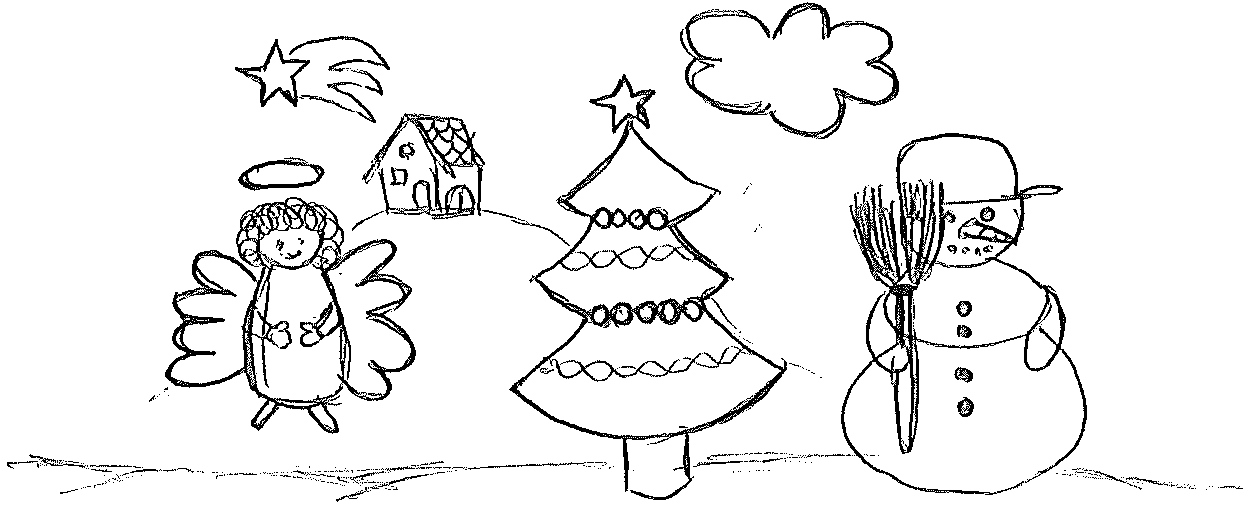
\includegraphics[scale=0.25]{/opt/share/90sek/Logos/Schneebild}} \\
%\vspace*{-11ex}
\\

}
\parbox[t]{.49\linewidth}{
 
\scriptsize
\textbf{\footnotesize \"Offnungszeiten}\\
Mo. -- Fr. \hfill{} 10\Uhr{} -- 14\Uhr{} Uhr\hspace*{1ex}\\
\vspace*{0.2ex}

\textbf{\footnotesize{Beratungs- und Servicezeiten}}\\
siehe Homepage\\

\textbf{\footnotesize AStA Sitzungen}\\
\scriptsize Fr. 14\Uhr{} Uhr (nat\"urlich \"offentlich!)\\

}

\vspace*{-1ex}

}





\footnotesize{\textbf{Impressum:} AStA der RWTH Aachen, Peterstra"se 44-46, 52062 Aachen}\\
\footnotesize{\textbf{ViSdP:} Johanna Sch"ope, \email{oeffentlichkeit@asta.rwth-aachen.de}}
	

		\end{minipage}
	}%fcolorbox
}

\vspace{-5ex}

%\begin{artikel}{Linkliste/Weitere Informationen}
\parbox{.1\linewidth}{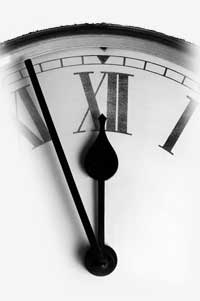
\includegraphics[width=\linewidth]{bilder/uhr}}
\parbox{.9\linewidth}{
\begin{aufzaehlung}
\item \url{www.asta.rwth-aachen.de} -- Webseiten des AStA mit aktuellen Infos und Sprechzeiten der BAf"oG-Beratung
\item \url{www.bafoeg.bmbf.de} -- Bundesministerium f�r Bildung und Forschung, Informationen und BAf"oG-Rechner
\item \url{www.studentenwerk-aachen.de} -- BAf"oG-Amt Aachen
\item \url{www.studis-online.de} und \url{www.bafoegrechner.de} -- aktuelle Infos rund ums BAf"oG
\end{aufzaehlung}}
\vspace*{1ex}

Der AStA bietet auch eine pers"onliche Beratung an. Die genauen Termine findest Du in der unten stehenden Kontaktbox oder auf unserer Webseite unter \url{www.asta.rwth-aachen.de/beratung}. Eine vorherige Terminabsprache ist nicht notwendig. Die Beratung ist kostenlos und erfolgt selbstverst"andlich vertraulich.
\end{artikel}

\end{rueckseite}
%<geschweifteKlammer>
\end{document}  


